\documentclass[14pt]{extbook}
\usepackage{multicol, enumerate, enumitem, hyperref, color, soul, setspace, parskip, fancyhdr} %General Packages
\usepackage{amssymb, amsthm, amsmath, latexsym, units, mathtools} %Math Packages
\everymath{\displaystyle} %All math in Display Style
% Packages with additional options
\usepackage[headsep=0.5cm,headheight=12pt, left=1 in,right= 1 in,top= 1 in,bottom= 1 in]{geometry}
\usepackage[usenames,dvipsnames]{xcolor}
\usepackage{dashrule}  % Package to use the command below to create lines between items
\newcommand{\litem}[1]{\item#1\hspace*{-1cm}\rule{\textwidth}{0.4pt}}
\pagestyle{fancy}
\lhead{Makeup Progress Quiz 2}
\chead{}
\rhead{Version A}
\lfoot{5763-3522}
\cfoot{}
\rfoot{Spring 2021}
\begin{document}

\begin{enumerate}
\litem{
Choose the graph of the equation below.\[ f(x) = \sqrt{x - 6} - 7 \]\begin{enumerate}[label=\Alph*.]
\begin{multicols}{2}\item 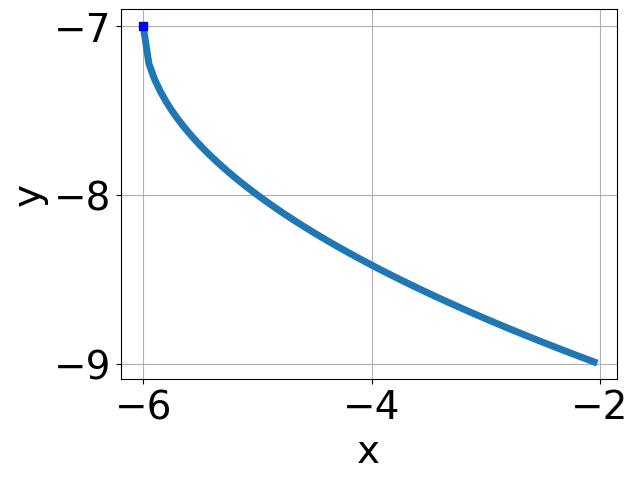
\includegraphics[width = 0.3\textwidth]{../Figures/radicalEquationToGraphAA.png}\item 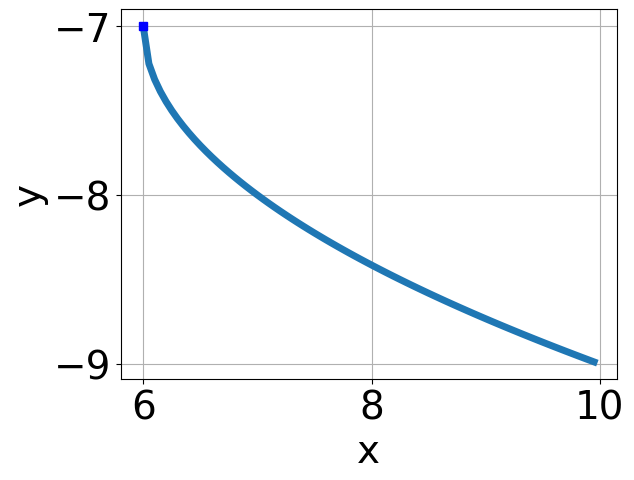
\includegraphics[width = 0.3\textwidth]{../Figures/radicalEquationToGraphBA.png}\item 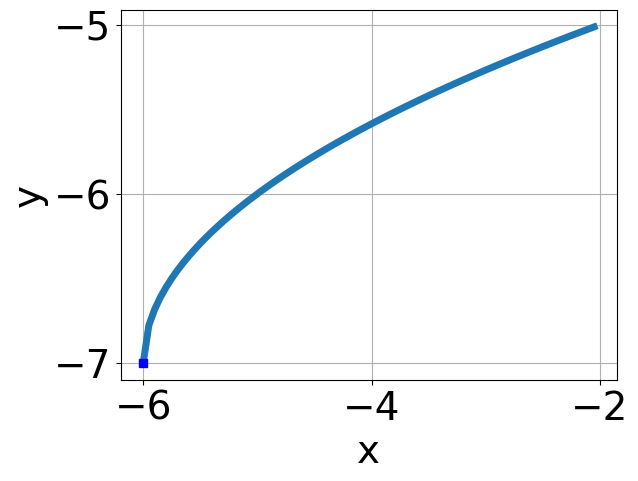
\includegraphics[width = 0.3\textwidth]{../Figures/radicalEquationToGraphCA.png}\item 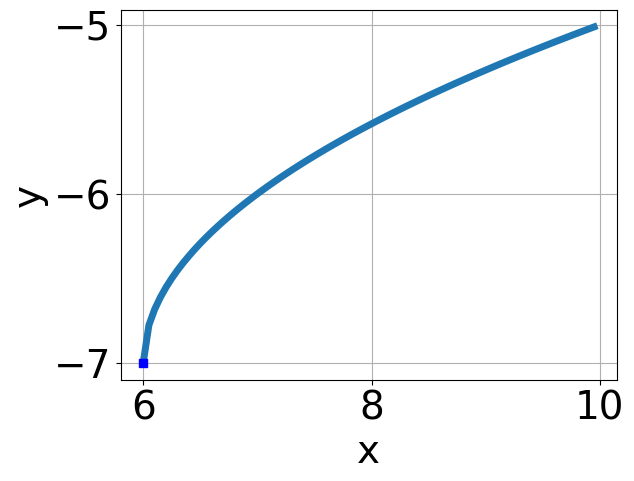
\includegraphics[width = 0.3\textwidth]{../Figures/radicalEquationToGraphDA.png}\end{multicols}\item None of the above.
\end{enumerate} }
\litem{
Choose the equation of the function graphed below.
\begin{center}
    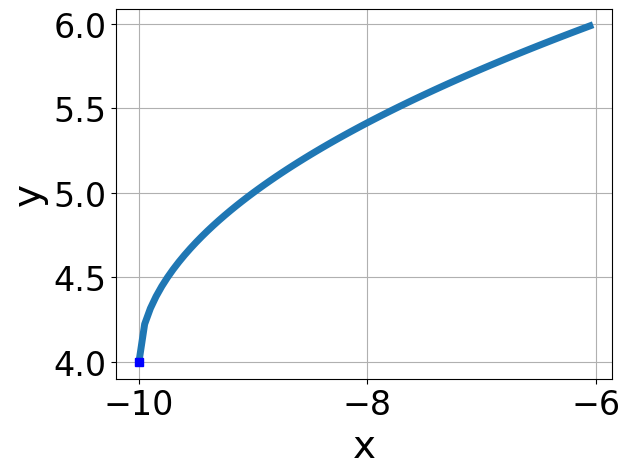
\includegraphics[width=0.5\textwidth]{../Figures/radicalGraphToEquationA.png}
\end{center}
\begin{enumerate}[label=\Alph*.]
\item \( f(x) = - \sqrt[3]{x + 10} + 4 \)
\item \( f(x) = \sqrt[3]{x - 10} + 4 \)
\item \( f(x) = \sqrt[3]{x + 10} + 4 \)
\item \( f(x) = - \sqrt[3]{x - 10} + 4 \)
\item \( \text{None of the above} \)

\end{enumerate} }
\litem{
Choose the graph of the equation below.\[ f(x) = - \sqrt[3]{x + 8} - 6 \]\begin{enumerate}[label=\Alph*.]
\begin{multicols}{2}\item 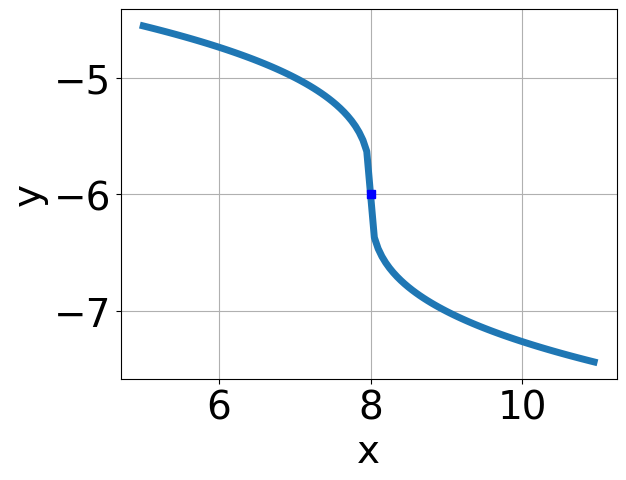
\includegraphics[width = 0.3\textwidth]{../Figures/radicalEquationToGraphCopyAA.png}\item 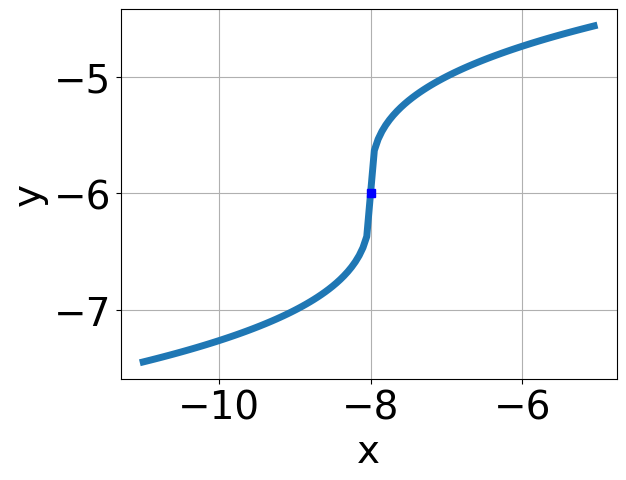
\includegraphics[width = 0.3\textwidth]{../Figures/radicalEquationToGraphCopyBA.png}\item 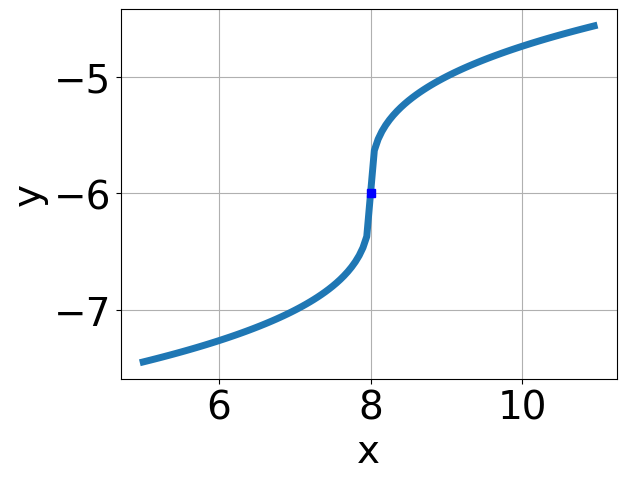
\includegraphics[width = 0.3\textwidth]{../Figures/radicalEquationToGraphCopyCA.png}\item 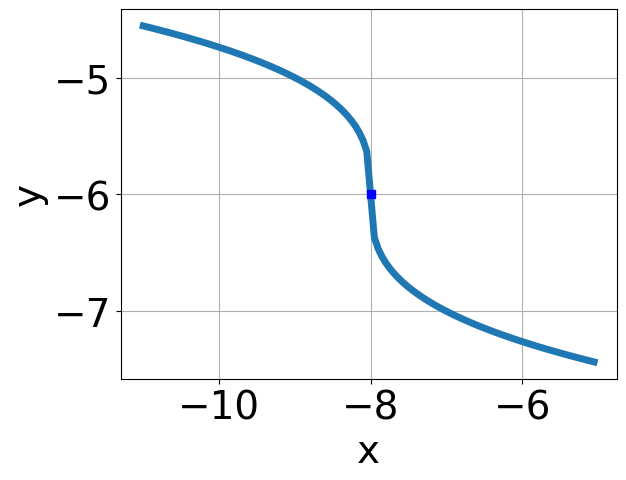
\includegraphics[width = 0.3\textwidth]{../Figures/radicalEquationToGraphCopyDA.png}\end{multicols}\item None of the above.
\end{enumerate} }
\litem{
What is the domain of the function below?\[ f(x) = \sqrt[5]{-6 x - 8} \]\begin{enumerate}[label=\Alph*.]
\item \( \text{The domain is } (-\infty, a], \text{   where } a \in [-0.82, 0.37] \)
\item \( \text{The domain is } (-\infty, a], \text{   where } a \in [-1.66, -0.89] \)
\item \( \text{The domain is } [a, \infty), \text{   where } a \in [-1.01, -0.49] \)
\item \( \text{The domain is } [a, \infty), \text{   where } a \in [-2.22, -0.94] \)
\item \( (-\infty, \infty) \)

\end{enumerate} }
\litem{
Solve the radical equation below. Then, choose the interval(s) that the solution(s) belongs to.\[ \sqrt{-24 x^2 - 36} - \sqrt{70 x} = 0 \]\begin{enumerate}[label=\Alph*.]
\item \( x \in [-2.9,-1.8] \)
\item \( x_1 \in [-2.9, -1.8] \text{ and } x_2 \in [-1.8,-0.5] \)
\item \( x \in [-2,0.9] \)
\item \( \text{All solutions lead to invalid or complex values in the equation.} \)
\item \( x_1 \in [0.8, 2.3] \text{ and } x_2 \in [-0.2,1.5] \)

\end{enumerate} }
\litem{
What is the domain of the function below?\[ f(x) = \sqrt[6]{-6 x - 9} \]\begin{enumerate}[label=\Alph*.]
\item \( [a, \infty), \text{where } a \in [-2.13, -0.77] \)
\item \( [a, \infty), \text{where } a \in [-0.89, 1.03] \)
\item \( (-\infty, \infty) \)
\item \( (-\infty, a], \text{ where } a \in [-3.3, -0.8] \)
\item \( (-\infty, a], \text{where } a \in [-1.3, -0.4] \)

\end{enumerate} }
\litem{
Solve the radical equation below. Then, choose the interval(s) that the solution(s) belongs to.\[ \sqrt{10 x^2 + 24} - \sqrt{32 x} = 0 \]\begin{enumerate}[label=\Alph*.]
\item \( x_1 \in [-2.26, -1.71] \text{ and } x_2 \in [-2.2,-0.2] \)
\item \( x_1 \in [0.88, 1.29] \text{ and } x_2 \in [1,4] \)
\item \( \text{All solutions lead to invalid or complex values in the equation.} \)
\item \( x \in [1.39,2.44] \)
\item \( x \in [0.88,1.29] \)

\end{enumerate} }
\litem{
Solve the radical equation below. Then, choose the interval(s) that the solution(s) belongs to.\[ \sqrt{8 x + 6} - \sqrt{-9 x - 9} = 0 \]\begin{enumerate}[label=\Alph*.]
\item \( x_1 \in [-0.98, -0.77] \text{ and } x_2 \in [-1.75,4.25] \)
\item \( x \in [0.13,0.26] \)
\item \( x_1 \in [-1.01, -0.96] \text{ and } x_2 \in [-1.75,4.25] \)
\item \( \text{All solutions lead to invalid or complex values in the equation.} \)
\item \( x \in [-0.98,-0.77] \)

\end{enumerate} }
\litem{
Solve the radical equation below. Then, choose the interval(s) that the solution(s) belongs to.\[ \sqrt{7 x - 7} - \sqrt{-4 x + 9} = 0 \]\begin{enumerate}[label=\Alph*.]
\item \( x \in [-0.4,0.27] \)
\item \( \text{All solutions lead to invalid or complex values in the equation.} \)
\item \( x \in [1.34,1.59] \)
\item \( x_1 \in [0.71, 1.1] \text{ and } x_2 \in [1.52,3.12] \)
\item \( x_1 \in [0.71, 1.1] \text{ and } x_2 \in [0.98,1.5] \)

\end{enumerate} }
\litem{
Choose the equation of the function graphed below.
\begin{center}
    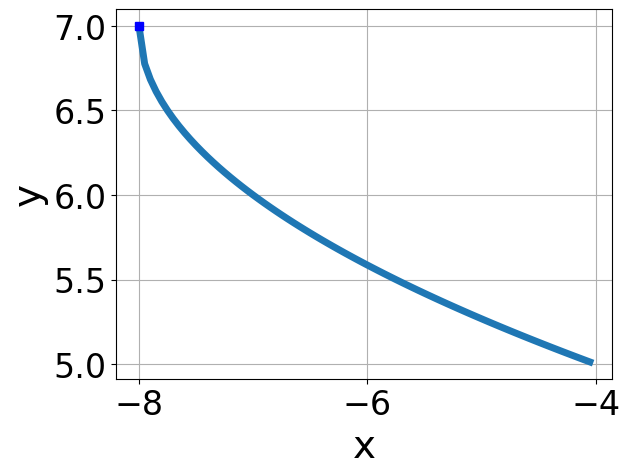
\includegraphics[width=0.5\textwidth]{../Figures/radicalGraphToEquationCopyA.png}
\end{center}
\begin{enumerate}[label=\Alph*.]
\item \( f(x) = \sqrt[3]{x - 8} + 7 \)
\item \( f(x) = \sqrt[3]{x + 8} + 7 \)
\item \( f(x) = - \sqrt[3]{x + 8} + 7 \)
\item \( f(x) = - \sqrt[3]{x - 8} + 7 \)
\item \( \text{None of the above} \)

\end{enumerate} }
\end{enumerate}

\end{document}